\documentclass{article}
\usepackage[utf8]{inputenc}
\usepackage{ffcode}
\usepackage{pgfplots}
\usepackage{hyperref}
\pgfplotsset{width=8cm,compat=1.9}

\def\dunderline#1{\underline{\underline{#1}}}

\title{Algoritmer og Datastrukturer Øving 3, alternativ 1}
\author{Nicolai H. Brand}
\date{September 2022}

\begin{document}

\maketitle

Kompiler og kjør programmet kan gjøres ved:
\begin{ffcode}
cc oblig3.c && ./a.out
\end{ffcode}

\section{Introduksjon}
Quicksort implementasjonen er tatt fra fagets undervisningsmateriell. Dual pivot quicksort implementasjon er hentet fra \hyperlink{geksforgeeks.com }{https://www.geeksforgeeks.org/dual-pivot-quicksort/}.

Målingene tatt for alle algoritmene er vedlagt som en del av den innsendte besvarelsen. Alle målingene ble tatt fra $n = 10 * 10^6$ til $n = 100 * 10^6$ med inkrement $i = 10 * 10^6$.

Det er skrevet en $sjekksum$ og en $rekkefølge$ test for å verifisere at listene inneholder de samme verdiene som før sorteringen, og at listene er blitt korrekt sortert.

\newpage

\section{Quicksort og dual pivot quicksort på ulike data}

\begin{center}
Tidsbruk til quicksort\\
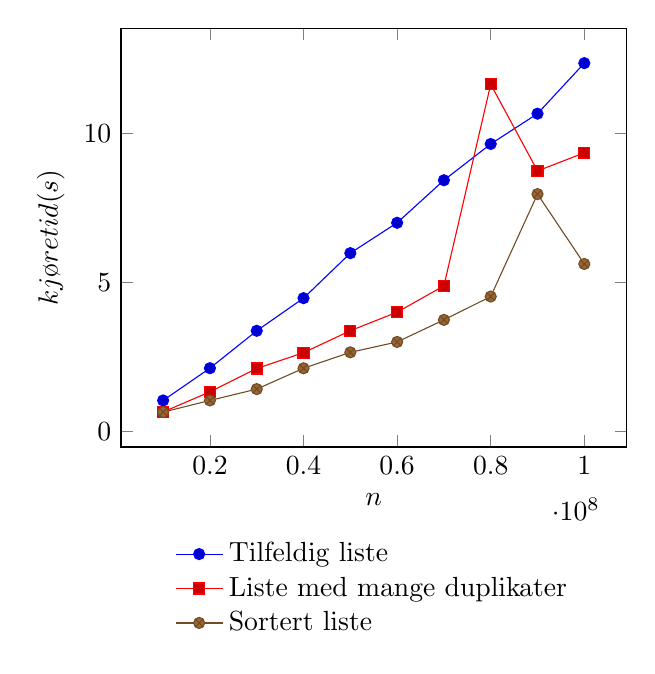
\begin{tikzpicture}
  \begin{axis}[
        xlabel = \(n\),
        ylabel = {\(kjøretid (s)\)},
        legend style={draw=none, nodes={scale=1, transform shape}, at={(0.5,-0.2)},anchor=north,legend cell align=left}
  ]
  
    %addlegendimage{empty legend style={at={(1,1)},anchor=west}}
    
    \addplot coordinates {
    (10000000, 1.040567)
    (20000000, 2.124645)
    (30000000, 3.380747)
    (40000000, 4.476836)
    (50000000, 5.989207)
    (60000000, 7.009237)
    (70000000, 8.438384)
    (80000000, 9.657051)
    (90000000, 10.674632)
    (100000000, 12.372759)
    };
    \addplot coordinates {
    (10000000, 0.654301)
    (20000000, 1.329104)
    (30000000, 2.114155)
    (40000000, 2.644632)
    (50000000, 3.383990)
    (60000000, 4.005473)
    (70000000, 4.890193)
    (80000000, 11.661463)
    (90000000, 8.752389)
    (100000000, 9.358601)
    };
    \addplot coordinates {
    (10000000, 0.648803)
    (20000000, 1.040693)
    (30000000, 1.421243)
    (40000000, 2.121394)
    (50000000, 2.656961)
    (60000000, 3.006198)
    (70000000, 3.746993)
    (80000000, 4.531565)
    (90000000, 7.972812)
    (100000000, 5.625212)
    };
    
    \addlegendentry{Tilfeldig liste}
    \addlegendentry{Liste med mange duplikater}
    \addlegendentry{Sortert liste}
  \end{axis}
\end{tikzpicture}
\end{center}

\begin{center}

Tidsbruk til dual pivot quicksort
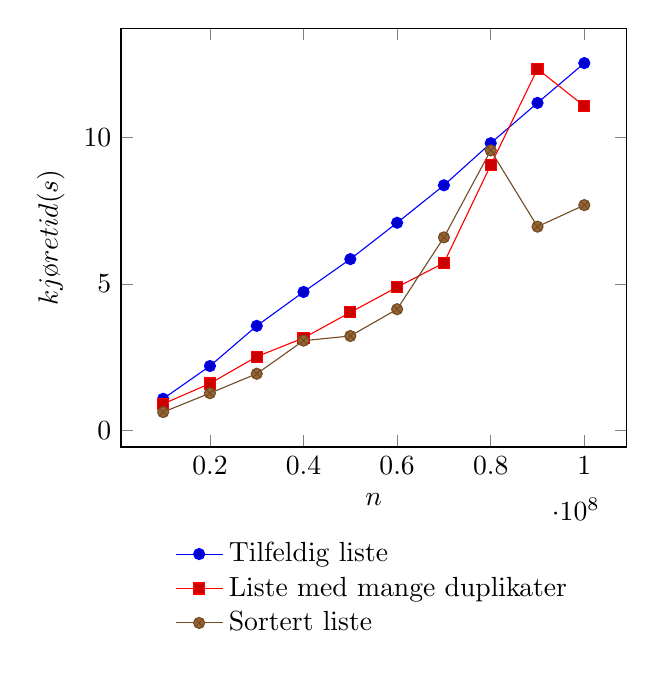
\begin{tikzpicture}
  \begin{axis}[
        xlabel = \(n\),
        ylabel = {\(kjøretid (s)\)},
        legend style={draw=none, nodes={scale=1, transform shape}, at={(0.5,-0.2)},anchor=north,legend cell align=left}
  ]

    \addplot coordinates {
    (10000000, 1.083661)
    (20000000, 2.202495)
    (30000000, 3.573021)
    (40000000, 4.730781)
    (50000000, 5.852240)
    (60000000, 7.092978)
    (70000000, 8.372321)
    (80000000, 9.809948)
    (90000000, 11.184699)
    (100000000, 12.542733)
    };
    
    \addplot coordinates {
    (10000000, 0.910098)
    (20000000, 1.604812)
    (30000000, 2.522031)
    (40000000, 3.161135)
    (50000000, 4.033308)
    (60000000, 4.894584)
    (70000000, 5.722623)
    (80000000, 9.062181)
    (90000000, 12.343138)
    (100000000, 11.075579)

    };
    \addplot coordinates {
    (10000000, 0.629342)
    (20000000, 1.275066)
    (30000000, 1.938540)
    (40000000, 3.068229)
    (50000000, 3.227638)
    (60000000, 4.142353)
    (70000000, 6.594367)
    (80000000, 9.563842)
    (90000000, 6.960026)
    (100000000, 7.695782)
    };
    
    \addlegendentry{Tilfeldig liste}
    \addlegendentry{Liste med mange duplikater}
    \addlegendentry{Sortert liste}
  \end{axis}
\end{tikzpicture}

\end{center}

\section{Sammenligning av quicksort og dual pivot quicksort}

\begin{center}
Sammenligning mellom quicksort og  dual pivot quicksort på tilfeldige lister
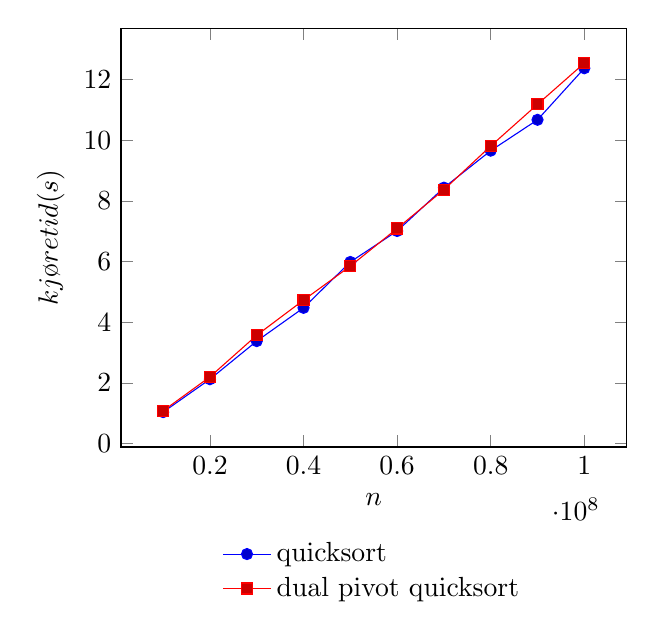
\begin{tikzpicture}
  \begin{axis}[
        xlabel = \(n\),
        ylabel = {\(kjøretid (s)\)},
        legend style={draw=none, nodes={scale=1, transform shape}, at={(0.5,-0.2)},anchor=north,legend cell align=left}
  ]
  
    \addplot coordinates {
    (10000000, 1.040567)
    (20000000, 2.124645)
    (30000000, 3.380747)
    (40000000, 4.476836)
    (50000000, 5.989207)
    (60000000, 7.009237)
    (70000000, 8.438384)
    (80000000, 9.657051)
    (90000000, 10.674632)
    (100000000, 12.372759)
    };
    \addplot coordinates {
    (10000000, 1.083661)
    (20000000, 2.202495)
    (30000000, 3.573021)
    (40000000, 4.730781)
    (50000000, 5.852240)
    (60000000, 7.092978)
    (70000000, 8.372321)
    (80000000, 9.809948)
    (90000000, 11.184699)
    (100000000, 12.542733)
    };
    
    \addlegendentry{quicksort}
    \addlegendentry{dual pivot quicksort}
  \end{axis}
\end{tikzpicture}
\end{center}


\begin{center}
Sammenligning mellom quicksort og  dual pivot quicksort på lister som inneholder mange duplikater
\\
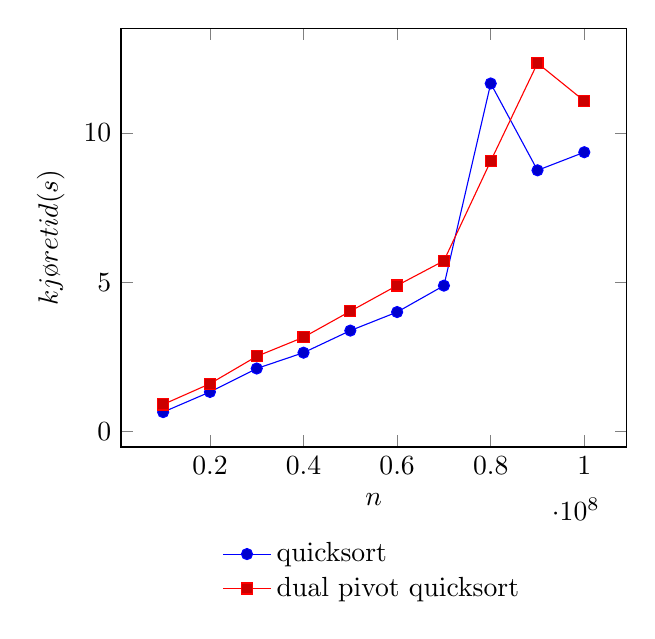
\begin{tikzpicture}
  \begin{axis}[
        xlabel = \(n\),
        ylabel = {\(kjøretid (s)\)},
        legend style={draw=none, nodes={scale=1, transform shape}, at={(0.5,-0.2)},anchor=north,legend cell align=left}
  ]
  
    \addplot coordinates {
    (10000000, 0.654301)
    (20000000, 1.329104)
    (30000000, 2.114155)
    (40000000, 2.644632)
    (50000000, 3.383990)
    (60000000, 4.005473)
    (70000000, 4.890193)
    (80000000, 11.661463)
    (90000000, 8.752389)
    (100000000, 9.358601)
    };
    \addplot coordinates {
    (10000000, 0.910098)
    (20000000, 1.604812)
    (30000000, 2.522031)
    (40000000, 3.161135)
    (50000000, 4.033308)
    (60000000, 4.894584)
    (70000000, 5.722623)
    (80000000, 9.062181)
    (90000000, 12.343138)
    (100000000, 11.075579)
    };
    
    \addlegendentry{quicksort}
    \addlegendentry{dual pivot quicksort}
  \end{axis}
\end{tikzpicture}
\end{center}

\begin{center}
Sammenligning mellom quicksort og dual pivot quicksort på lister som allerede er sortert.
\\
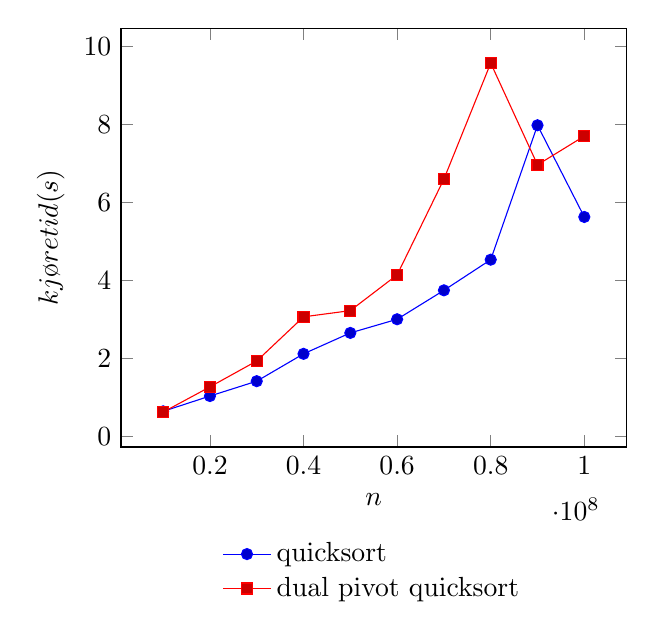
\begin{tikzpicture}
  \begin{axis}[
        xlabel = \(n\),
        ylabel = {\(kjøretid (s)\)},
        legend style={draw=none, nodes={scale=1, transform shape}, at={(0.5,-0.2)},anchor=north,legend cell align=left}
  ]
  
    \addplot coordinates {
    (10000000, 0.648803)
    (20000000, 1.040693)
    (30000000, 1.421243)
    (40000000, 2.121394)
    (50000000, 2.656961)
    (60000000, 3.006198)
    (70000000, 3.746993)
    (80000000, 4.531565)
    (90000000, 7.972812)
    (100000000, 5.625212)
    };
    \addplot coordinates {
    (10000000, 0.629342)
    (20000000, 1.275066)
    (30000000, 1.938540)
    (40000000, 3.068229)
    (50000000, 3.227638)
    (60000000, 4.142353)
    (70000000, 6.594367)
    (80000000, 9.563842)
    (90000000, 6.960026)
    (100000000, 7.695782)
    };
    
    \addlegendentry{quicksort}
    \addlegendentry{dual pivot quicksort}
  \end{axis}
\end{tikzpicture}
\end{center}

\section{Diskusjon}
Jevnt over alle tilfellene bruker quicksort marginalt mindre tid en dual pivot quicksort. Dette strider med forventningen at dual pivot quicksort er en forbedring av quicksort. Dual pivot quicksort er en mer omstendig og intrikat algoritme som resulterer at den er mer følsom for implementasjonsdetaljer. Det kan tenkes at implementasjonen hentet fra \hyperlink{geksforgeeks.com }{https://www.geeksforgeeks.org/dual-pivot-quicksort/} ikke er optimal.

Begge algoritmene blir raskere på mer gunstig datasett. Selv om tidskompleksiteten til begge algoritmene er \(n * log(n)\) blir tidskompleksiteten tilnærmet \(n\) for store verdier av \(n\).

\end{document}
